Dans cette section, nous allons analyser les principales solutions existantes, qu'elles soient 
sous la forme d'applications utilisateur ou intégrées directement dans un système d'exploitation (\acrshort{os}).
Jean-Francois Dockes en dresse également une liste avec avantages et inconvénients sur son site 
\cite{ref3}. Ce que nous recherchons est une application \textit{open source}, fonctionnant sur Linux, 
stockant les tags dans les \textit{extended attributes} (\acrshort{xattr}), ne modifiant pas les fichiers et performante.

%%%%%%%%%%%%%%%%%%%%%%%%%%%%%%%%%%%%%%%%%%%%%%%%%%%%%%%%%%%%%%%%%%%%%%%%%%%%%%%%%%%%%%%%%%%%%%%%%%%
%%%%%%%%%%%%%%%%%%%%%%%%%%%%%%%%%%%%%%%%%%%%%%%%%%%%%%%%%%%%%%%%%%%%%%%%%%%%%%%%%%%%%%%%%%%%%%%%%%%
\subsection{Applications utilisateur}
%%%%%%%%%%%%%%%%%%%%%%%%%%%%%%%%%%%%%%%%%%%%%%%%%%%%%%%%%%%%%%%%%%%%%%%%%%%%%%%%%%%%%%%%%%%%%%%%%%%
%%%%%%%%%%%%%%%%%%%%%%%%%%%%%%%%%%%%%%%%%%%%%%%%%%%%%%%%%%%%%%%%%%%%%%%%%%%%%%%%%%%%%%%%%%%%%%%%%%%
\subsubsection{TMSU}
TMSU \cite{ref15} est un outil en ligne de commande (\acrshort{cli}) qui permet d'attribuer des tags à des 
fichiers et d'exécuter des recherches par tags. On commence par initialiser TMSU dans le répertoire choisi. 
Une commande liste les tags associés à un ou 
plusieurs fichiers et une autre liste les fichiers qui possèdent le ou les tags donnés. TMSU offre 
la possibilité à l'utilisateur de "monter" un système de fichiers (\acrshort{fs}) virtuel avec FUSE (Filesystem in 
UserSpacE). L'outil est rapide et efficace, mais il comporte quelques défauts :
\begin{itemize}
    \item Pas d'interface graphique.
    \item Dépendance à FUSE pour monter le \acrshort{fs} virtuel.
    \item Stockage des tags dans une base de données SQLite : si la base est perdue, les tags le sont également.
\end{itemize}

%%%%%%%%%%%%%%%%%%%%%%%%%%%%%%%%%%%%%%%%%%%%%%%%%%%%%%%%%%%%%%%%%%%%%%%%%%%%%%%%%%%%%%%%%%%%%%%%%%%
%%%%%%%%%%%%%%%%%%%%%%%%%%%%%%%%%%%%%%%%%%%%%%%%%%%%%%%%%%%%%%%%%%%%%%%%%%%%%%%%%%%%%%%%%%%%%%%%%%%
\subsubsection{Tagsistant}
Tagsistant \cite{ref16} est autre outil en ligne de commande (\acrshort{cli}) de gestion de tags. Il dépend de FUSE et d'une base 
de données (SQLite ou MySQL) pour fonctionner. Comme pour TMSU, il faut donner un répertoire à Tagsistant 
pour son usage interne. À l'intérieur de ce dernier, se trouvent différents répertoires :
\dirtree{%
.1 /.
.2 alias --- Répertoire contenant les requêtes les plus courantes.
.2 archive --- Répertoire listant les fichiers.
.2 relations --- Répertoire contenant les relations entre les tags et fichiers.
.2 stats --- Répertoire contenant des infos sur l'utilisation de Tagsistant.
.2 store --- Répertoire où sont gérés les fichiers et ajoutés les tags.
.2 tags --- Répertoire de gestion des tags.
}
\bigbreak
Chaque répertoire a un rôle bien précis. Tout se fait avec le terminal et des commandes usuelles 
(\mintinline{text}{cp}, \mintinline{text}{ls}, \mintinline{text}{mkdir}, etc.). Dans Tagsistant, 
un répertoire créé dans le répertoire \mintinline{text}{tags} correspond à un tag. On se retrouve 
finalement avec une arborescence de tags et de fichiers \cite{ref17}. Bien que cet outil soit 
performant d'un point de vue de la rapidité d'exécution, il comporte les défauts de TMSU ainsi que 
des nouveaux :
\begin{itemize}
    \item Pas d'interface graphique.
    \item Dépendance à FUSE pour monter le \acrshort{fs} virtuel.
    \item Stockage des tags dans une base de données : si la base est perdue, les tags le sont également.
    \item Utilisation des différents répertoires peu intuitive.
    \item Tous les fichiers sont contenus dans un seul répertoire et leur nom est modifié pour les 
        besoins internes de l'application. Obligation de passer par l'application pour accéder aux 
        fichiers.
\end{itemize} 

%%%%%%%%%%%%%%%%%%%%%%%%%%%%%%%%%%%%%%%%%%%%%%%%%%%%%%%%%%%%%%%%%%%%%%%%%%%%%%%%%%%%%%%%%%%%%%%%%%%
%%%%%%%%%%%%%%%%%%%%%%%%%%%%%%%%%%%%%%%%%%%%%%%%%%%%%%%%%%%%%%%%%%%%%%%%%%%%%%%%%%%%%%%%%%%%%%%%%%%
\subsubsection{TaggedFrog}
TaggedFrog \cite{ref18} est un programme disponible sur Windows uniquement et ne partage pas ses sources.
Son fonctionnement interne n'est pas documenté. L'interface est agréable, on peut ajouter des fichiers 
par \textit{Drag \& Drop}. L'interface créé au fur et à mesure un "nuage" de tags, comme on peut le retrouver sur 
certains sites web. On peut exécuter des recherches sur les tags et les fichiers. On peut supposer que 
TaggedFrog maintient une base de données des tags associés aux fichiers, ce qui ne correspond à nouveau 
pas à nos besoins.
\begin{figure}
    \begin{center}
        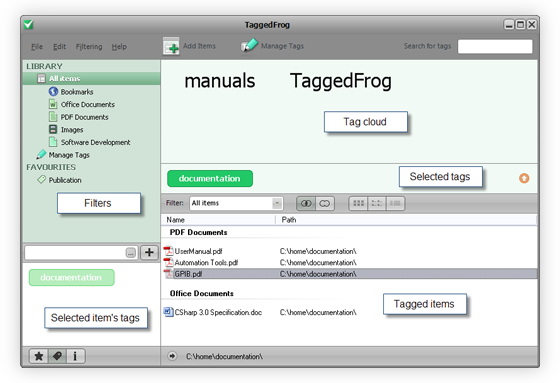
\includegraphics[width=0.8\textwidth]{images/taggedfrog.png}
    \end{center}
    \caption{TaggedFrog en utilisation \cite{ref18}}
    \label{taggedfrog}
\end{figure}

%%%%%%%%%%%%%%%%%%%%%%%%%%%%%%%%%%%%%%%%%%%%%%%%%%%%%%%%%%%%%%%%%%%%%%%%%%%%%%%%%%%%%%%%%%%%%%%%%%%
%%%%%%%%%%%%%%%%%%%%%%%%%%%%%%%%%%%%%%%%%%%%%%%%%%%%%%%%%%%%%%%%%%%%%%%%%%%%%%%%%%%%%%%%%%%%%%%%%%%
\subsubsection{TagSpaces}
TagSpaces \cite{ref13} est un programme avec une interface graphique (\acrshort{gui}) permettant 
d'étiqueter ses fichiers avec des tags. 
L'application est agréable à utiliser, on commence par connecter un emplacement qui fera office de répertoire de 
destination aux fichiers. On peut ajouter ou créer des fichiers depuis l'application. Les fichiers 
existants ajoutés depuis l'application sont copiés dans le répertoire (cela créé donc un doublon). 
Sur le panneau de gauche se situe la zone de gestion des tags. TagSpaces ajoute automatiquement 
certains tags dits "intelligents" aux fichiers nouvellement créés avec l'application (par exemple 
un tag avec la date de création).
\begin{figure}
    \begin{center}
        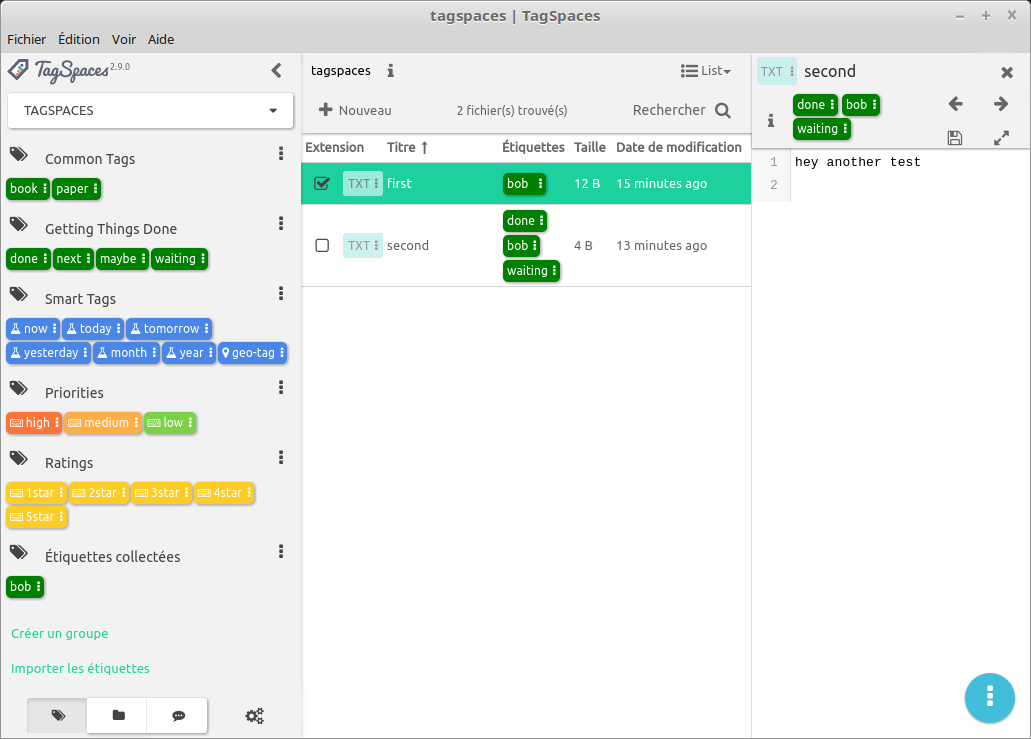
\includegraphics[width=0.8\textwidth]{images/tagspaces.png}
    \end{center}
    \caption{TagSpaces en utilisation}
    \label{tagspaces}
\end{figure}
Globalement, l'application est fonctionnelle et \textit{user friendly}. Cependant, deux points noirs 
sont à déplorer :
\begin{enumerate}
    \item L'application copie les fichiers déjà existants sélectionnés par l'utilisateur, ce qui 
        créé une contrainte supplémentaire dans la gestion de ses fichiers personnels.
    \item TagSpaces stocke les tags directement dans le nom du fichier, modifiant ainsi son nom \cite{ref14}.
        Bien que pratique dans le cas d'une synchronisation à l'aide d'un service cloud, 
        le fichier devient dépendant de TagSpaces. Si l'utilisateur décide de changer son nom sans 
        respecter la nomenclature interne, il risque de perdre les tags associés au fichier.
\end{enumerate}

%%%%%%%%%%%%%%%%%%%%%%%%%%%%%%%%%%%%%%%%%%%%%%%%%%%%%%%%%%%%%%%%%%%%%%%%%%%%%%%%%%%%%%%%%%%%%%%%%%%
%%%%%%%%%%%%%%%%%%%%%%%%%%%%%%%%%%%%%%%%%%%%%%%%%%%%%%%%%%%%%%%%%%%%%%%%%%%%%%%%%%%%%%%%%%%%%%%%%%%
\subsection{Fonctionnalités disponibles dans l'\acrshort{os}}

%%%%%%%%%%%%%%%%%%%%%%%%%%%%%%%%%%%%%%%%%%%%%%%%%%%%%%%%%%%%%%%%%%%%%%%%%%%%%%%%%%%%%%%%%%%%%%%%%%%
%%%%%%%%%%%%%%%%%%%%%%%%%%%%%%%%%%%%%%%%%%%%%%%%%%%%%%%%%%%%%%%%%%%%%%%%%%%%%%%%%%%%%%%%%%%%%%%%%%%
\subsubsection{Windows}
À partir de Windows Vista, Microsoft a donné la possibilité aux utilisateurs d'ajouter des 
méta-données aux fichiers; parmi ces méta-données se trouvent les tags. Il existe une fonctionnalité 
appelée \textit{Search Folder} qui permet de créer un répertoire virtuel contenant le résultat d'une 
recherche sur les noms de fichiers ou d'autres critères \cite{ref19}. Depuis Windows 8, l'utilisateur 
a la possibilité d'ajouter des méta-données à certains types de fichiers (ceux de la suite office 
par exemple), dont des tags. Il peut par la suite exécuter des recherches ciblées via 
l'explorateur de fichiers Windows du type \mintinline{text}{meta:value} \cite{ref20}. C'est 
dommage que Windows ne prenne pas en compte davantage de types de fichiers, comme les PDFs ou les 
fichiers \mintinline{text}{.txt}.

%%%%%%%%%%%%%%%%%%%%%%%%%%%%%%%%%%%%%%%%%%%%%%%%%%%%%%%%%%%%%%%%%%%%%%%%%%%%%%%%%%%%%%%%%%%%%%%%%%%
%%%%%%%%%%%%%%%%%%%%%%%%%%%%%%%%%%%%%%%%%%%%%%%%%%%%%%%%%%%%%%%%%%%%%%%%%%%%%%%%%%%%%%%%%%%%%%%%%%%
\subsubsection{macOS}\label{existant_macOS}
macOS possède son propre système pour étiqueter des fichiers. Il est intégré depuis la version 
OS X 10.9 Mavericks. Depuis l'explorateur de fichiers, l'utilisateur a la possibilité 
d'ajouter, modifier, supprimer et rechercher des tags. Les fichiers peuvent avoir plusieurs tags 
associés. Un code couleur permet de plus facilement se souvenir et visualiser les tags attribués. 
Dans l'explorateur de fichiers, les tags se retrouvent sur le bas côté, pour y accéder plus 
rapidement. 
\begin{figure}
    \begin{center}
        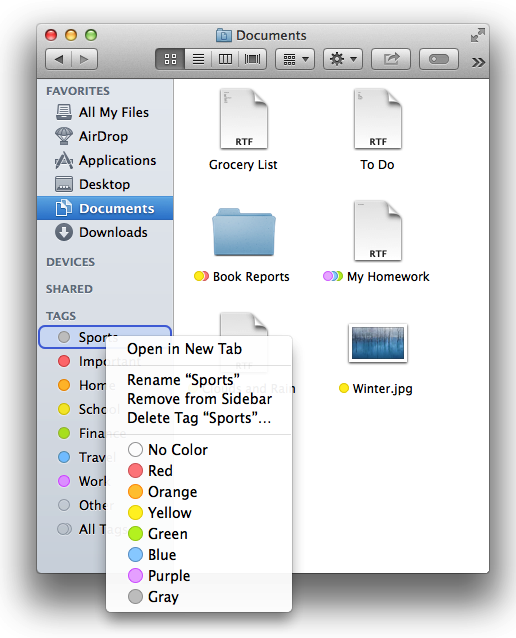
\includegraphics[width=0.55\textwidth]{images/macos_tags.png}
    \end{center}
    \caption{Vue et gestion d'un tag dans le Finder macOS \cite{ref5}}
    \label{macos_tags}
\end{figure}
Lorsque l'on clique sur un tag, une recherche Spotlight est effectuée. Spotlight est le moteur de 
recherche interne à macOS. Spotlight garde un index des tags, fournissant un accès rapide aux 
fichiers correspondants \cite{ref9}.
Tous ces tags peuvent se synchroniser sur les différents "iDevices" via iCloud. Finalement, 
un menu de réglages permet la gestion des tags (affichage, suppression, etc.) \cite{ref5}, 
\cite{ref6}. L'implémentation de ce système utilise les \acrshort{xattr} pour stocker les tags. 
Les différents tags se trouvent dans l'attribut \mintinline{shell}{kMDItemUserTags}, listés les 
uns à la suite des autres. Via le Terminal, à l'aide de la commande \mintinline{shell}{mdls}, 
nous pouvons afficher la liste des tags associés à un fichier, nommé "Hello" pour l'exemple :
\bigbreak
\begin{code}
    \begin{minted}[bgcolor=mygray,breaklines,breaksymbol=,linenos,frame=single,stepnumber=1,tabsize=2]{shell}
% mdls -name kMDItemUserTags Hello 
kMDItemUserTags = (
    Green,
    Red,
    Essential
)
    \end{minted}
    \caption{\mintinline{shell}{mdls} listant les tags d'un fichier sous macOS \cite{ref7}}
\end{code}
\bigbreak
Ici, le fichier \mintinline{text}{Hello} est étiqueté avec trois tags, "Green", "Red" et "Essential". Le fait que 
l'indexation est réalisée avec Spotlight implique une réindexation des fichiers dans le cas d'un 
changement de nom pour un tag donné sous macOS. Le framework système \mintinline{text}{FSEvents} 
donne une solution partielle : c'est une \acrshort{api} (utilisée également par Spotlight) qui offre aux 
applications la possibilité d'être notifiées si un changement a eu lieu sur un répertoire (un événement 
toutes les 30 secondes). \mintinline{text}{FSEvents} maintient des logs de ces changements dans 
des fichiers, les applications peuvent ainsi retrouver l'historique des changements quand elles 
le souhaitent \cite{ref10}. Les seuls points négatifs de cette implémentation, c'est qu'elle 
n'est pas \textit{open source}, qu'elle n'existe que sur macOS et qu'elle n'est pas écrite en Rust. 
Mais c'est la solution vers laquelle ce projet essaie de se rapprocher car elle correspond aux 
critères sur les \acrshort{xattr} et le fonctionnement interne.
